\documentclass[12pt,a4paper]{article}
\usepackage{tikz}
\usetikzlibrary{arrows.meta,positioning}
\usepackage{tabularx}
\usepackage{graphicx}
\usepackage{amsmath}
\usepackage{amssymb}
\usepackage{amsthm}
\usepackage{bm}
\usepackage{hyperref}
\usepackage{booktabs}
\usepackage{array}
\usepackage{geometry}
\geometry{margin=2.5cm}
\hypersetup{colorlinks=true, linkcolor=blue, citecolor=blue, urlcolor=blue}
\newtheorem{theorem}{Theorem}
\newtheorem{proposition}{Proposition}
\newtheorem{definition}{Definition}
\newtheorem{lemma}{Lemma}
\newtheorem{corollary}{Corollary}
\newtheorem{criterion}{Criterion}




\title{\textbf{Paper A-03: Earth Ocean Currents:\\ A Constraint-Driven Flux Dynamics (CDFD) Perspective}}
\author{Steve Bico Mujjabi, MD\\
\small Independent Researcher\\
\small Founder, Vura Labs\\
\small Kampala, Uganda\\
\small ORCID: 0009-0001-0556-5516}
\date{May 2026}


\newcommand{\EarthSuppPath}{Part\_A\_Earth\_Systems/supplementary/supplementary\_earth\_}
\newcommand{\EngSuppPath}{Part\_B\_Engineered\_Systems/supplementary/supplementary\_eng\_}
\newcommand{\SocSuppPath}{Part\_C\_Socioeconomic\_Systems/supplementary/supplementary\_soc\_}
\newcommand{\DomainSuppPath}{Part\_D\_Domain\_Applications/supplementary/supplementary\_dom\_}
\begin{document}
\maketitle

\begin{abstract}
This paper treats ocean currents as a CDFD/AFL modelling hypothesis. Wind
stress, buoyancy forcing, heat, salt, and mass transport are read as fluxes
$\Phi$ moving through basin geometry, stratification, bathymetry, mixing limits,
and freshwater constraints $C$. The claim is not that CDFD/AFL replaces
physical oceanography. The claim is that the notation can organise measurable
questions about transport, bottlenecks, responsiveness, and long memory in the
ocean system.
\end{abstract}

\section*{Symbol Conventions}

\noindent\textbf{CDFD/AFL Part IV symbol convention.}
\begin{center}
{\small
\begin{tabular}{p{0.15\linewidth}p{0.34\linewidth}p{0.41\linewidth}}
\hline
Symbol & Part IV meaning & Cross-domain reading \\
\hline
$\Phi$ & Driving flux or throughput & Energy, matter, signal, capital, information, traffic, force, or biological load entering a system \\
$C$ & Active constraint or capacity burden & Bottleneck, resistance, boundary, scarcity, toxicity, regulation, topology, latency, or load-bearing limit \\
$S$ & Responsiveness or adaptive surface & The system's ability to reconfigure, buffer, route, repair, learn, or preserve function under changing load \\
$M_s$ & Structural memory & Stored damage, hysteresis, inherited topology, institutional memory, trained weights, ecological legacy, or retained state \\
$\Psi_s$ & Adaptive operating ratio $(\Phi/C)\cdot S\cdot M_s$ & Local bookkeeping gauge for constrained operation, overload, recovery, or regime change; not a universal constant \\
$\Lambda$ & Life Number or capstone surplus ratio where explicitly defined & Reserved for Part II-derived life-number notation or synthesis-level surplus measures, never an undefined decoration \\
\hline
\end{tabular}
}
\end{center}

\noindent\textbf{Greek-symbol convention.}
\begin{center}
{\small
\begin{tabular}{p{0.15\linewidth}p{0.34\linewidth}p{0.41\linewidth}}
\hline
Symbol & Local role & Interpretation rule \\
\hline
$\alpha$ & Accumulation or reinforcement coefficient & Sets how fast a pathway, constraint, habit, cascade, or retained structure grows under load \\
$\beta$ & Relaxation, decay, clearance, or washout coefficient & Sets loss, recovery, damping, forgetting, degradation, or return toward baseline \\
$\gamma$ & Coupling, diffusion, redistribution, or transfer coefficient & Sets spread across nodes, layers, tissues, markets, infrastructures, media, or physical phases \\
$\delta,\epsilon$ & Perturbation, tolerance, small offset, or numerical guard & Used only as local thresholds, stability margins, measurement tolerances, or stress increments \\
$\eta,\lambda,\mu,\nu$ & Efficiency, rate, baseline, intensity, or frequency terms & Meaning is fixed by the equation, subscript, and domain-specific proxy in the paragraph where the term appears \\
$\rho,\sigma,\tau,\phi$ & Density/correlation, variability/noise, time-scale, phase, or field terms & Local coefficients only; subscripts bind them to the named pathway, domain, or experiment \\
$\Omega,\Lambda$ & Domain/state space; Life Number where defined & $\Omega$ names a modeled state space; $\Lambda$ carries life-number or synthesis notation only when the paper defines it \\
\hline
\end{tabular}
}
\end{center}

\section{Series Context}

Part I sets the flow--constraint language used here \cite{MujjabiPartI2026}.
Part II develops the Life Number and the origins-of-life use of the same notation
\cite{MujjabiPartII2026}. Part III applies AFL to biology and medicine
\cite{MujjabiPartIII2026}. Part IV \cite{MujjabiPartIV2026}, DOI \url{https://doi.org/10.5281/zenodo.20395901}, uses the language as a cross-domain stress
test, with measurement kept separate from analogy.

\section{Ocean Transport Frame}

The ocean stores and redistributes heat, salt, carbon, nutrients, and momentum.
Its flow is constrained by basin walls, seafloor geometry, density structure,
wind forcing, sea ice, freshwater input, and mixing depth. In the CDFD/AFL
reading, a current system is not only a velocity field; it is a flow path with
capacity, inertia, adaptive response, and memory.

\section{Candidate Variable Map}

\begin{table}[h]
\centering
\begin{tabularx}{\textwidth}{@{}lXX@{}}
\toprule
CDFD term & Ocean-current reading & Example proxy \\
\midrule
$\Phi$ & ocean transport or forcing & Sverdrup transport, heat flux, freshwater flux \\
$C$ & active constraint & stratification, bathymetry, sill depth, friction \\
$S$ & responsiveness & mixing, eddy compensation, current-path adjustment \\
$M_s$ & structural memory & heat storage, salinity anomaly, overturning inertia \\
$\Psi_s$ & operating ratio & balanced, constrained, stalled, or amplified transport \\
\bottomrule
\end{tabularx}
\end{table}

\section{Memory and Circulation Change}

Ocean memory is central to the mapping. Heat stored below the mixed layer,
persistent salinity anomalies, ice-ocean feedback, and overturning inertia can
make present circulation depend on prior forcing. In CDFD/AFL terms, high
$M_s$ means the current state carries a record of earlier flux and constraint.
That does not by itself prove a new mechanism; it gives a way to state what
must be measured.

\section{Measurement Layer}

A useful ocean application specifies the current system, the forcing window,
the proxy for $\Phi$, the constraint term $C$, the response term $S$, and the
memory term $M_s$. Candidate failure conditions include persistent transport
weakening, blocked heat redistribution, salinity-driven stratification, or a
shift in overturning regime. The mapping has value only if it improves
measurement or interpretation beyond ordinary oceanographic diagnostics.

\section{Current Runtime Diagnostic}

The Part E diagnostic run includes an ocean-transport adapter row and the
universal cascade stress test. These outputs check finite runtime behavior in
the current CDFD Runtime \cite{CDFDRuntime2026}. They do not validate any ocean
claim; they record model behavior that later data work can test.

\section{Tests That Can Break the Mapping}

The ocean-current mapping weakens if the chosen proxies for flux, constraint,
responsiveness, and memory do not track observed transport changes; if a
standard ocean model explains the same behavior more cleanly; or if the CDFD
terms cannot be tied to reproducible ocean data.

% BEGIN PART IV MAJOR UNIVERSAL UPGRADE
\section{Major Universal Upgrade: Mechanism, Scale, and Tests}

\subsection{Observable Translation}

The paper-specific translation begins with an observable chain rather than a
verbal analogy. For Earth Ocean Currents, the proposed drive is wind stress, buoyancy forcing, tides, and freshwater input.
The active limitation is bathymetry, stratification, friction, and mixing limits. Responsiveness is carried by
eddies, overturning, mixing, and boundary-current adjustment, while retained state is represented by
heat, salinity, oxygen, and circulation history. The outcome to explain is heat transport, ventilation, current strength, and recovery.

\begin{table}[htbp]
\centering
\small
\caption{Operational CDFD/AFL map for Paper A-03.}
\begin{tabularx}{\textwidth}{|l|X|X|}
\hline
\textbf{Term} & \textbf{Paper-specific observable meaning} & \textbf{Measurement question} \\
\hline
$\Phi$ & wind stress, buoyancy forcing, tides, and freshwater input & What rate, load, gradient, or demand enters the focal system? \\
\hline
$C$ & bathymetry, stratification, friction, and mixing limits & Which measured bottleneck limits transfer, function, or recovery? \\
\hline
$S$ & eddies, overturning, mixing, and boundary-current adjustment & Which process changes effective capacity or reroutes the load? \\
\hline
$M_s$ & heat, salinity, oxygen, and circulation history & Which retained state makes equal present loads produce different futures? \\
\hline
$Y$ & heat transport, ventilation, current strength, and recovery & Which outcome is predicted out of sample, with uncertainty? \\
\hline
\end{tabularx}
\end{table}

\begin{figure}[htbp]
\centering
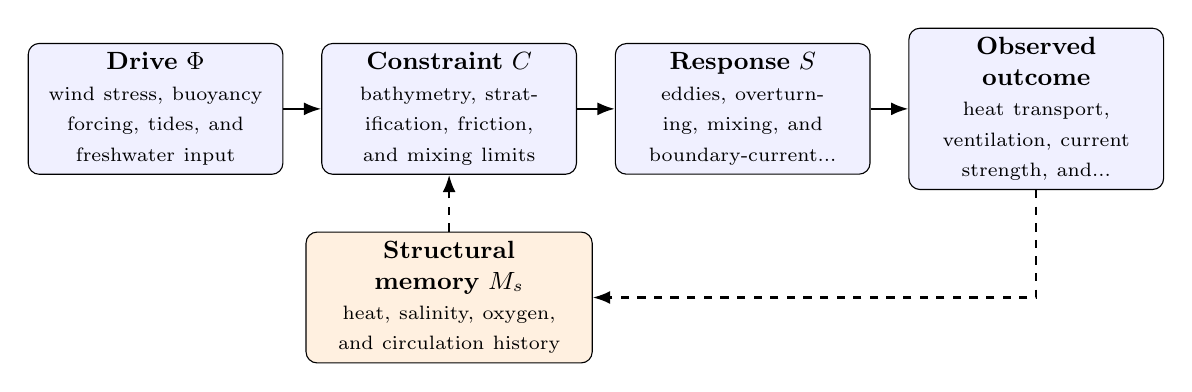
\begin{tikzpicture}[
    node distance=0.48cm,
    every node/.style={font=\small},
    box/.style={draw, rounded corners, align=center, minimum height=1.45cm, text width=3.0cm, fill=blue!6},
    memory/.style={draw, rounded corners, align=center, minimum height=1.25cm, text width=3.4cm, fill=orange!12},
    flow/.style={-{Latex[length=2.2mm]}, thick},
    feedback/.style={-{Latex[length=2.2mm]}, thick, dashed}
]
\node[box] (drive) {\textbf{Drive $\Phi$}\\\scriptsize wind stress, buoyancy forcing, tides, and freshwater input};
\node[box, right=of drive] (constraint) {\textbf{Constraint $C$}\\\scriptsize bathymetry, stratification, friction, and mixing limits};
\node[box, right=of constraint] (response) {\textbf{Response $S$}\\\scriptsize eddies, overturning, mixing, and boundary-current...};
\node[box, right=of response] (outcome) {\textbf{Observed outcome}\\\scriptsize heat transport, ventilation, current strength, and...};
\node[memory, below=0.72cm of constraint] (memory) {\textbf{Structural memory $M_s$}\\\scriptsize heat, salinity, oxygen, and circulation history};
\draw[flow] (drive) -- (constraint);
\draw[flow] (constraint) -- (response);
\draw[flow] (response) -- (outcome);
\draw[feedback] (outcome.south) |- (memory.east);
\draw[feedback] (memory.north) -- (constraint.south);
\end{tikzpicture}
\caption{Paper A-03 observable CDFD/AFL architecture for Earth Ocean Currents. Solid arrows give the proposed forward chain; dashed arrows make history-dependent feedback explicit.}
\label{fig:a03-architecture}
\end{figure}

\subsection{Minimal Coupled Model}

A paper-level model must separate throughput, constraint accumulation, response,
and history. One deliberately minimal form is
\begin{align}
Y(t) &= \frac{\Phi(t)S(t)}{\epsilon + C(t)}, \\
\frac{dC}{dt} &= \alpha \Phi(t) - \beta S(t)C(t) + \gamma \mathcal{L}C(t), \\
\frac{dM_s}{dt} &= \eta C(t) - \mu M_s(t), \\
\Psi_s(t) &= \frac{\widehat{\Phi}(t)}{\epsilon+\widehat{C}(t)}\,
             \widehat{S}(t)\,[1+\omega\widehat{M_s}(t)] .
\end{align}
Here $Y$ is the measured output, $\epsilon>0$ prevents a singular denominator,
$\mathcal{L}$ is a spatial or network coupling operator, and hats denote
explicitly normalized variables. The sign and magnitude of $\omega$ must be
estimated: memory can preserve useful organization or amplify damage. No fixed
threshold is universal before the variables, normalization, and observation
scale are declared.

For this paper, the hypothesized causal sequence is specific. A change in
wind stress, buoyancy forcing, tides, and freshwater input arrives faster than eddies, overturning, mixing, and boundary-current adjustment can compensate.
This raises or redistributes bathymetry, stratification, friction, and mixing limits. If the load persists,
the retained state encoded by heat, salinity, oxygen, and circulation history changes the next response, so a later event of equal
magnitude can produce a different trajectory in heat transport, ventilation, current strength, and recovery. The
scientific task is to estimate that sequence against the best ordinary model of
the domain, not merely to redescribe the outcome after it occurs.

\subsection{Cross-Scale Universality Without Mechanistic Erasure}

For the Earth systems family, the universal comparison is between coupled transport, finite environmental capacity, buffering, and retained landscape or ecosystem state. Universality here cannot erase conservation laws, geometry, or scale; it must expose where those domain equations create comparable overload and recovery structures. \cite{Holling1973,Turing1952,BakTangWiesenfeld1987}
The CDFD programme is cumulative: Part I supplies the flow--constraint
foundation \cite{MujjabiPartI2026}; Part II asks when maintained throughput
supports persistent organized states \cite{MujjabiPartII2026}; Part III
develops adaptive limitation and biological memory \cite{MujjabiPartIII2026};
and Part IV \cite{MujjabiPartIV2026} tests how much of that architecture
survives translation. The CDFD Runtime \cite{CDFDRuntime2026} supplies a
reproducible numerical stress surface, but it does not substitute for the
domain evidence named here.

The required scale declaration for this paper is hours to centuries; turbulence to global overturning. At short
scales, the key question is whether the incoming drive is transmitted,
buffered, or diverted. At intermediate scales, response changes effective
capacity and network exposure. At long scales, retained structure can alter the
state space itself. A result is genuinely cross-scale only when the aggregation
rule is stated and the same conclusion is not an artifact of averaging.

\subsection{Evidence Ladder and Discriminating Tests}

\begin{table}[htbp]
\centering
\small
\caption{Evidence ladder for Paper A-03. Each rung can fail independently.}
\begin{tabularx}{\textwidth}{|p{0.17\textwidth}|X|X|}
\hline
\textbf{Test} & \textbf{Design} & \textbf{Discriminating result} \\
\hline
Proxy audit & Measure Argo profiles, altimetry, moorings, tracers, and hydrography and preregister how each record maps to $\Phi$, $C$, $S$, $M_s$, and $Y$. & The mapping fails if proxies are non-identifiable, circular, or change meaning across cases. \\
\hline
Load ramp & Apply or observe a freshwater or heat pulse applied to a stratified basin while estimating the dominant constraint and response time. & A threshold claim requires a reproducible nonlinear change and uncertainty bounds, not a visually chosen breakpoint. \\
\hline
Recovery and memory & Match present load across units with different histories, then compare recovery paths. & The memory claim requires history-dependent divergence after current conditions are controlled. \\
\hline
Model comparison & Compare the baseline domain model with and without the CDFD/AFL state variables using held-out data. & The paper's stated falsifier is: the CDFD variables add no out-of-sample skill beyond ocean circulation models. \\
\hline
\end{tabularx}
\end{table}

The strongest practical design combines a prospective perturbation with a
recovery window. The load-ramp phase estimates where constraint begins to rise
faster than output. The recovery phase estimates $\beta$ and $\mu$, separating
fast relaxation from persistent memory. A topology or coupling intervention
then asks whether rerouting changes the cascade as predicted. Null results are
informative because they identify domains in which the universal notation adds
no measurable value.

\subsection{Research Programme and Boundary Conditions}

The immediate research programme has four steps. First, construct a documented
dataset from Argo profiles, altimetry, moorings, tracers, and hydrography and retain raw units before normalization.
Second, fit a baseline domain model and report its calibration and out-of-sample
error. Third, add the smallest identifiable CDFD/AFL state extension and test
whether it improves prediction of heat transport, ventilation, current strength, and recovery. Fourth, repeat the
analysis across the declared scale range and publish negative cases as part of
the universality audit.

Three boundaries are non-negotiable. Correlation between flow and failure does
not identify a constraint mechanism. A fitted memory term does not prove that
the stored state has the same material meaning in another domain. Finally, a
runtime cascade is evidence about the implementation, not evidence that the
real system follows it. The paper becomes stronger when it can say precisely
where the translation stops.


% END PART IV MAJOR UNIVERSAL UPGRADE

\section{Conclusion}

Ocean-current observations provide a direct test of flow, constraint, response,
and memory. The CDFD and AFL framing is useful here only as a disciplined
measurement language, and the release-level claim remains limited to that role.

\section*{Conflict of Interest}
The author declares no conflict of interest.

\section*{Data Availability}
Part-specific runtime diagnostics are under each Part's \path{outputs/} directory.

Release-wide code: \path{Part_E_Synthesis/supplementary/}.

Generated summaries: \path{Part_E_Synthesis/outputs/}.

Figures: \path{Part_E_Synthesis/figures/}.


\section{Reference Layer}

\bibliographystyle{plain}
\bibliography{universal_afl_references}
\end{document}
